\documentclass[11pt,preprint, authoryear]{elsarticle}


\usepackage{lmodern}
%%%% My spacing
\usepackage{setspace}
\setstretch{1.2}
\DeclareMathSizes{12}{14}{10}{10}

% Wrap around which gives all figures included the [H] command, or places it "here". This can be tedious to code in Rmarkdown.
\usepackage{float}
\let\origfigure\figure
\let\endorigfigure\endfigure
\renewenvironment{figure}[1][2] {
    \expandafter\origfigure\expandafter[H]
} {
    \endorigfigure
}

\let\origtable\table
\let\endorigtable\endtable
\renewenvironment{table}[1][2] {
    \expandafter\origtable\expandafter[H]
} {
    \endorigtable
}


\usepackage{ifxetex,ifluatex}
\usepackage{fixltx2e} % provides \textsubscript
\ifnum 0\ifxetex 1\fi\ifluatex 1\fi=0 % if pdftex
  \usepackage[T1]{fontenc}
  \usepackage[utf8]{inputenc}
\else % if luatex or xelatex
  \ifxetex
    \usepackage{mathspec}
    \usepackage{xltxtra,xunicode}
  \else
    \usepackage{fontspec}
  \fi
  \defaultfontfeatures{Mapping=tex-text,Scale=MatchLowercase}
  \newcommand{\euro}{€}
\fi

\usepackage{amssymb, amsmath, amsthm, amsfonts}

\def\bibsection{\section*{References}} %%% Make "References" appear before bibliography


\usepackage[round]{natbib}

\usepackage{longtable}
\usepackage[margin=2.3cm,bottom=2cm,top=2.5cm, includefoot]{geometry}
\usepackage{fancyhdr}
\usepackage[bottom, hang, flushmargin]{footmisc}
\usepackage{graphicx}
\numberwithin{equation}{section}
\numberwithin{figure}{section}
\numberwithin{table}{section}
\setlength{\parindent}{0cm}
\setlength{\parskip}{1.3ex plus 0.5ex minus 0.3ex}
\usepackage{textcomp}
\renewcommand{\headrulewidth}{0pt}

\usepackage{array}
\newcolumntype{x}[1]{>{\centering\arraybackslash\hspace{0pt}}p{#1}}

%%%%  Remove the "preprint submitted to" part. Don't worry about this either, it just looks better without it:
\makeatletter
\def\ps@pprintTitle{%
  \let\@oddhead\@empty
  \let\@evenhead\@empty
  \let\@oddfoot\@empty
  \let\@evenfoot\@oddfoot
}
\makeatother

 \def\tightlist{} % This allows for subbullets!

\usepackage{hyperref}
\hypersetup{breaklinks=true,
            bookmarks=true,
            colorlinks=true,
            citecolor=blue,
            urlcolor=blue,
            linkcolor=blue,
            pdfborder={0 0 0}}


% The following packages allow huxtable to work:
\usepackage{siunitx}
\usepackage{multirow}
\usepackage{hhline}
\usepackage{calc}
\usepackage{tabularx}
\usepackage{booktabs}
\usepackage{caption}


\newenvironment{columns}[1][]{}{}

\newenvironment{column}[1]{\begin{minipage}{#1}\ignorespaces}{%
\end{minipage}
\ifhmode\unskip\fi
\aftergroup\useignorespacesandallpars}

\def\useignorespacesandallpars#1\ignorespaces\fi{%
#1\fi\ignorespacesandallpars}

\makeatletter
\def\ignorespacesandallpars{%
  \@ifnextchar\par
    {\expandafter\ignorespacesandallpars\@gobble}%
    {}%
}
\makeatother

\newlength{\cslhangindent}
\setlength{\cslhangindent}{1.5em}
\newenvironment{CSLReferences}%
  {\setlength{\parindent}{0pt}%
  \everypar{\setlength{\hangindent}{\cslhangindent}}\ignorespaces}%
  {\par}


\urlstyle{same}  % don't use monospace font for urls
\setlength{\parindent}{0pt}
\setlength{\parskip}{6pt plus 2pt minus 1pt}
\setlength{\emergencystretch}{3em}  % prevent overfull lines
\setcounter{secnumdepth}{5}

%%% Use protect on footnotes to avoid problems with footnotes in titles
\let\rmarkdownfootnote\footnote%
\def\footnote{\protect\rmarkdownfootnote}
\IfFileExists{upquote.sty}{\usepackage{upquote}}{}

%%% Include extra packages specified by user

%%% Hard setting column skips for reports - this ensures greater consistency and control over the length settings in the document.
%% page layout
%% paragraphs
\setlength{\baselineskip}{12pt plus 0pt minus 0pt}
\setlength{\parskip}{12pt plus 0pt minus 0pt}
\setlength{\parindent}{0pt plus 0pt minus 0pt}
%% floats
\setlength{\floatsep}{12pt plus 0 pt minus 0pt}
\setlength{\textfloatsep}{20pt plus 0pt minus 0pt}
\setlength{\intextsep}{14pt plus 0pt minus 0pt}
\setlength{\dbltextfloatsep}{20pt plus 0pt minus 0pt}
\setlength{\dblfloatsep}{14pt plus 0pt minus 0pt}
%% maths
\setlength{\abovedisplayskip}{12pt plus 0pt minus 0pt}
\setlength{\belowdisplayskip}{12pt plus 0pt minus 0pt}
%% lists
\setlength{\topsep}{10pt plus 0pt minus 0pt}
\setlength{\partopsep}{3pt plus 0pt minus 0pt}
\setlength{\itemsep}{5pt plus 0pt minus 0pt}
\setlength{\labelsep}{8mm plus 0mm minus 0mm}
\setlength{\parsep}{\the\parskip}
\setlength{\listparindent}{\the\parindent}
%% verbatim
\setlength{\fboxsep}{5pt plus 0pt minus 0pt}



\begin{document}



\begin{frontmatter}  %

\title{Modelling Tobacco Demand: How the Illicit Cigarette Market
Constrains the Legal Market}

% Set to FALSE if wanting to remove title (for submission)




\author[Add1]{Cassandra Pengelly}
\ead{}





\address[Add1]{Stellenbosch University}



\vspace{1cm}





\vspace{0.5cm}

\end{frontmatter}



%________________________
% Header and Footers
%%%%%%%%%%%%%%%%%%%%%%%%%%%%%%%%%
\pagestyle{fancy}
\chead{}
\rhead{Thesis Draft}
\lfoot{}
\rfoot{}
\lhead{}
%\rfoot{\footnotesize Page \thepage } % "e.g. Page 2"
\cfoot{}

%\setlength\headheight{30pt}
%%%%%%%%%%%%%%%%%%%%%%%%%%%%%%%%%
%________________________

\headsep 35pt % So that header does not go over title




The main aim of the study is to investigate the relationship between the
legal and illegal tobacco market in South Africa. The study intends to:

\begin{itemize}
\item
  Define the legal and illegal tobacco market
\item
  Model tobacco demand
\item
  Estimate price elasticities
\item
  Understand whether the illegal tobacco market constrains the legal
  market
\end{itemize}

According to (\protect\hyperlink{ref-FATF}{\textbf{FATF?}}), the
definition of illicit trading of tobacco products is: ``\ldots the
supply, distribution and sale of smuggled genuine, counterfeit, or cheap
white tobacco products\ldots{}'' where smuggling is conducted to avoid
excise taxes, and/or to evade rules prohibiting the sale of such goods.
As (\protect\hyperlink{ref-Saenz}{\textbf{Saenz?}}) acknowledge, one of
the difficulties in investigating and modelling tobacco is deciding how
to measure illicit trade, given the limits on the availability of data.
These authors suggest that researchers studying illicit trade should
cross-validate their estimates using different methods.

This paper will measure the illicit market by two different methods. The
first method defines the illicit market by price: if a pack of
cigarettes is sold for less than the sum of the excise duty and VAT,
then it follows that it has been sold illegally. The logic being that
there is no economic incentive to sell packs at a loss, which suggests
that if a pack is being sold at less than its tax amount, tax is not
being paid on the cigarettes and they are thus illegal. The second
method defines the illicit market by volume: the illegal market is the
difference between the tax that should be paid on the total cigarette
packs produced and sold, and the actual tax paid.

Following a similar approach as
(\protect\hyperlink{ref-Bos}{\textbf{Bos?}}), a vector autoregression
will be used to estimate the long run elasticities of cigarette
consumption. The proposed base model is described by \ref{eq1}

\begin{align}
 Q_t = \mu + \sum_{i = 1}^{n}\beta_iQ_{t-i} +\sum_{i = 1}^{n}\gamma_iP_{t-i} + \sum_{i = 1}^{n}\theta_iY_{t-i} + \sum_{i = 1}^{n}\phi_iI_{t-i} \label{eq1}
\end{align}

where \(Q_t\) is the log of cigarette consumption,\newline \(P_{t}\) is
the log of real cigarette price,\newline \(Y_{t}\) is the log of real
disposable income,\newline \(I_{t}\) is the log of real illicit
cigarette price,\newline \(n\) is the number of lags and t is measured
in months

\hypertarget{data}{%
\section{\texorpdfstring{Data \label{dat}}{Data }}\label{data}}

The sample period for this study runs from January 2012 to March 2020.
Monthly data is used such that there are 99 observation points for each
variable in the data set. One of the advantages of using monthly data
rather than annual data is that it allows for more degrees of freedom.
The data used includes figures for the prices and volumes of cigarettes
in South Africa, tobacco excise duties, VAT, and disposable income. To
prepare the data for analysis the most popular price category (MPPC) was
identified as the 20-cigarette pack. Then a weighted average of
before-tax 20-pack prices was used as a base price. The excise duty per
20's pack and VAT and were then added to the base price to calculate the
price of licit cigarettes. The licit, illicit and disposable income
amounts were adjusted for inflation, taking December 2016 as the base
month and year. All of the variables have been transformed into log
form.

The figure below \ref{plot1} plots the time series of the logged
variables. The graphs show that the data could be trending, which is
formally tested in section \ref{Meth}.

\begin{figure}

{\centering \includegraphics{Thesis_Draft_files/figure-latex/Figure2-1} 

}

\caption{Time Series Plot \label{plot1}}\label{fig:Figure2}
\end{figure}

\hypertarget{methodology}{%
\section{\texorpdfstring{Methodology
\label{Meth}}{Methodology }}\label{methodology}}

To check whether the data is stationary, a number of tests is employed.
First the autocorrelation functions are plotted below \ref{plot2}. They
indicate that all four series are persistent; this is confirmed by the
Ljung-Box tests in table \ref{box}. The Ljung-Box test for independence
assesses whether there is significant evidence for non-zero correlations
at a given lag, with the null hypothesis that there is independence in a
given time series. A low p-value indicates a signal of non-stationarity.
The augmented Dickey Fuller test (\ref {adf}) suggests that all four of
the series contain a unit root (using the number of lags as
10\footnote{Some of the series test as stationary when the number of
  lags is reduced}. This further suggests that the series are
non-stationary.

\begin{figure}
\centering
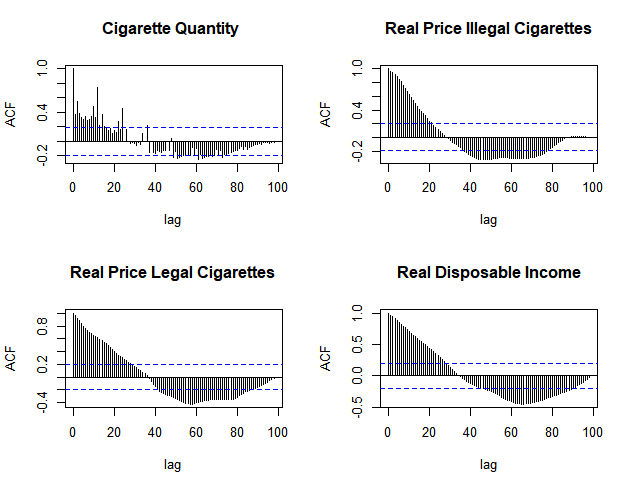
\includegraphics{img/ACF.png}
\caption{\label{plot2} ACF Plots}
\end{figure}

\begin{table}[H]
\centering
\begin{tabular}{lrll}
  \hline
Time Series & p value & Test Result & Interpretation \\ 
  \hline
Cigarette Quantity & 0.00 & Reject Null & Non-stationary \\ 
  Real Price Legal & 0.00 & Reject Null & Non-stationary \\ 
  Real Price Illegal & 0.00 & Reject Null & Non-stationary \\ 
  Real Disposable Income & 0.00 & Reject Null & Non-stationary \\ 
   \hline
\end{tabular}
\caption{Ljung-Box Test \label{box}} 
\end{table}

\begin{table}[H]
\centering
\begin{tabular}{lrll}
  \hline
Time Series & p value & Test Result & Interpretation \\ 
  \hline
Cigarette Quantity & 0.61 & Fail to reject Null & Non-stationary \\ 
  Real Price Legal & 0.22 & Fail to reject Null & Non-stationary \\ 
  Real Price Illegal & 0.38 & Fail to reject Null & Non-stationary \\ 
  Real Disposable Income & 0.06 & Fail to reject Null & Non-stationary \\ 
   \hline
\end{tabular}
\caption{Augmented Dickey-Fuller Test \label{adf}} 
\end{table}

To assess whether a long-run relationship between the variables exists,
the Johansen test is employed. According to Akaike's information
criterion (AIC), the appropriate maximum number of lags to use is 10
(\ref{lag}). A lag order of 9 is used for the test, since the test
requires a lag order of N - 1 = 10 - 1 = 9. Two Johansen tests are used:
the Trace and the Maximum Eigenvalue tests. The Trace statistic test
(\ref{coint}) shows we reject the null hypothesis that there are zero
cointegrating relationships: the test statistic 85.85 is greater than
the 1\% significance level of 55.43. The test results indicate that
there is 1 cointegrating relationship. Similarly, the Maximum Eigenvalue
test rejects that there are zero cointegrating relationships, and fails
to reject that there is at most 1 cointegrating relationship. The
presence of a cointegrating vector amongst the variables suggests a
Vector Error Correction Model is appropriate to analyse the variable
dynamics.

\begin{table}[H]
\centering
\begin{tabular}{rrrr}
  \hline
AIC(n) & HQ(n) & SC(n) & FPE(n) \\ 
  \hline
 10 &   5 &   2 &  10 \\ 
   \hline
\end{tabular}
\caption{Optimal Lag Selection \label{lag}} 
\end{table}

\begin{table}[H]
\centering
\begin{tabular}{rrrrr}
  \hline
 & Test Statistic & 10\% & 5\% & 1\% \\ 
  \hline
r$<$=3 & 1.21 & 6.50 & 8.18 & 11.65 \\ 
  r$<$=2 & 6.04 & 15.66 & 17.95 & 23.52 \\ 
  r$<$=1 & 26.89 & 28.71 & 31.52 & 37.22 \\ 
  r=0 & 85.85 & 45.23 & 48.28 & 55.43 \\ 
   \hline
\end{tabular}
\caption{Johansen Trace Test for Cointegration Results\label{coint}} 
\end{table}
\begin{table}[H]
\centering
\begin{tabular}{rrrrr}
  \hline
 & Test Statistic & 10\% & 5\% & 1\% \\ 
  \hline
r$<$=3 & 1.21 & 6.50 & 8.18 & 11.65 \\ 
  r$<$=2 & 4.83 & 12.91 & 14.90 & 19.19 \\ 
  r$<$=1 & 20.85 & 18.90 & 21.07 & 25.75 \\ 
  r=0 & 58.95 & 24.78 & 27.14 & 32.14 \\ 
   \hline
\end{tabular}
\caption{Johansen Eigenvalue Test for Cointegration Results\label{eigen}} 
\end{table}

A summary of the VECM results is given in \ref{vecm1}. The full model
output with 9 lags

\begin{longtable}{rll}
  \hline
 & ECT & Intercept \\ 
  \hline
QDP & -1.9701(0.5869)**  & 0.0054(0.0238)     \\ 
  PREALWAPDP & 0.0598(0.0301).   & -0.0022(0.0012).   \\ 
  PREALWAPDNP & -0.1659(0.1979)     & 0.0100(0.0080)     \\ 
  YDISPREAL & 0.0078(0.0081)     & 0.0001(0.0003)     \\ 
   \hline
\hline
\caption{Vector Error Correction Model 2SLS\label{vecm1}} 
\end{longtable}
\begin{longtable}{rllll}
  \hline
 & QDP-1 & PREALWAPDP-1 & PREALWAPDNP-1 & YDISPREAL-1 \\ 
  \hline
QDP & 0.7123(0.5286)     & -6.5487(2.6841)*   & 0.5219(0.5503)     & 12.7417(10.2110)     \\ 
  PREALWAPDP & -0.0565(0.0271)*   & 0.0007(0.1375)     & 0.0567(0.0282)*   & 0.9735(0.5229).   \\ 
  PREALWAPDNP & 0.1705(0.1783)     & 0.5743(0.9052)     & -0.2648(0.1856)     & -1.8064(3.4435)     \\ 
  YDISPREAL & -0.0078(0.0073)     & 0.0229(0.0369)     & 0.0093(0.0076)     & 0.8393(0.1406)*** \\ 
   \hline
\hline
\caption{Vector Error Correction Model 2SLS\label{vecm11}} 
\end{longtable}

\hypertarget{diagnostic-tests}{%
\subsection{Diagnostic Tests}\label{diagnostic-tests}}

TO test the accuracy of the model, a number of diagnostic tests were
run. \newpage

\hypertarget{appendix}{%
\section{\texorpdfstring{Appendix
\label{app}}{Appendix }}\label{appendix}}

\bibliography{Tex/ref}





\end{document}
